%
%	Begrifflichkeiten
%

\pagebreak
\section{Data definition and wrangling}

\onehalfspacing

\subsection{The Blog}

\subsection{Plausible}

In a previous paper, I have covered Plausible in more detail and compared it with other web analytics tools\footnote{See \textit{Frank, C. (2020)}: Usefulness of open-source tools for web analytics in E-Marketing.\cite{previousPaper}}; I will not go any further into details of the tool itself in this paper. As we will see later, it would be a good alternative to wp-statistics, which is used for the KFF blog

\begin{figure}[H]
\centering
\caption {Plausible}
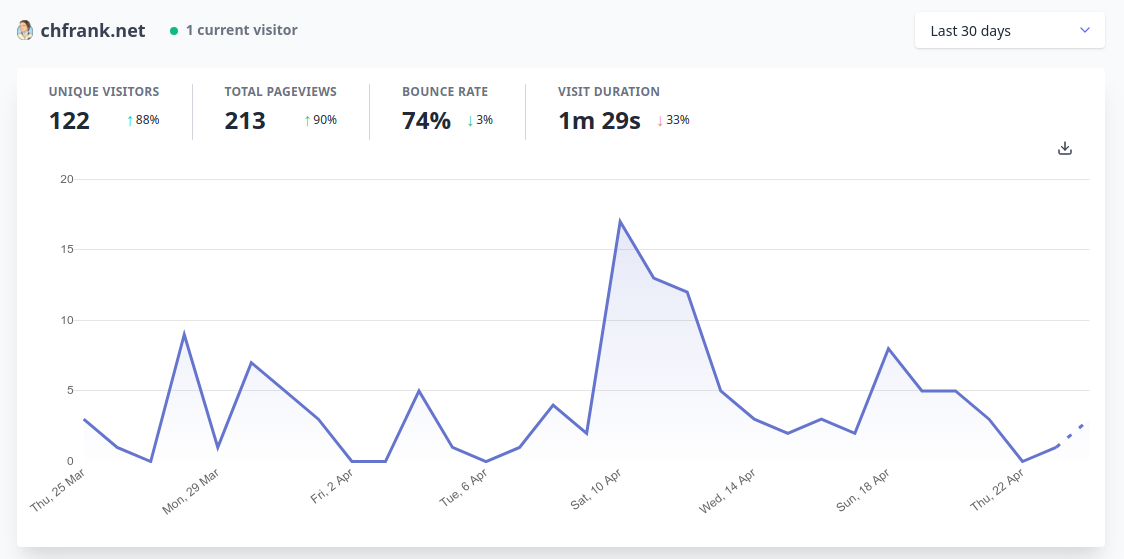
\includegraphics[width=\linewidth]{images/plausible.png}
\label{fig:plausible}
\end{figure}

\subsection{Count}

To analyze and visualize the data, I'll be using data notebooks from Count. Like Jupyter notebooks that combine (Python) Code and Text, the data notebooks combine (SQL) Data and Text in a pretty ingenious way. Data notebooks support data-driven decision making, and have recently come out of open beta.\footnote{See \textit{Count.co (2020)}: About Count.\cite{aboutCount}}

\subsection{Web Traffic KPIs}

In marketing categories, a blog belongs to inbound marketing, as it tries to offer engaging content and create value for the visitors but does not reach out by itself. 

Unlike outbound email campaigns, for example, that ask the visitor to view a particular website, a blog relies on its content and the willingness of the visitor to actively choose the site for a visit, for example, by being pointed to a post from a Google search result or a tweet.

In WordPress, there is an option to subscribe to a blog to get a notification on new posts; WordPress also provides the ability to subscribe to a blog's RSS feed. Even though, as this requires active user interaction and interest, blogs are considered an inbound channel.

In a recent paper on inbound marketing, Yvonne Romes identifies a couple of important KPIs for inbound marketing, a couple of which I will summarize here based on her paper:\footnote{See \textit{Romes, Y. (2020)}: 10 Inbound KPIs, die jetzt auch Personaler kennen sollten.\cite{inboundKPI}}

\begin{itemize}
\item Page Views
\item Bounce Rate
\item Visit Duration
\item Unique Visitors
\end{itemize}

Page Views is the number of clicks a specific page has received; on a blog, more page views indicate more engaging content.

Bounce Rate describes the rate of users that leave the site without selecting another link; a high bounce rate can indicate a lack of engaging or interesting content.

Visit Duration is the amount of time a unique visitor spends on the website; for a blog that mainly offers content to read, a longer duration most likely indicates higher engagement.

A unique visitor is a visitor that can be differentiated from another visitor. Unlike many other platforms, Plausible does not use tracking cookies to identify individual visitors but relies on publicly available information, such as an IP address, to differentiate them. Even though the metric is less accurate with Plausible than with other platforms, it's still an important metric, and as before, on a blog, more visitors usually indicate higher engagement.

In this paper, these are the four metrics that I will focus on.

\subsection{Social Media and Loneliness}

In the current COVID-19 pandemic, social distancing is a key element in containing the virus's spread. Social distancing over a long period of time can increase loneliness and significantly affect people's health negatively, according to a recent study conducted by the American Psychological Association.\footnote{See \textit{Luchetti, M. (2020)}: The trajectory of loneliness in response to COVID-19. \cite{apaLoneliness}}

In the study, the researchers formulate the hypothesis that an increase in perceived support from others can offset loneliness during the required isolation.

One element to offset the effects of loneliness is increased interaction on social media and virtual meetings with video. Social media interaction includes reading blogs - the more engaging a blog post is, the more chances it has to reach people to whom it will be entertaining or otherwise beneficial.

Thus this analysis aims to get an answer for my blog on the question "On which subject(s) should I post to increase my reach?". We will be using visualization and correlation as the primary means of analysis to increase the value of the blog for others.

\subsection{Data Collection}

Data exported from the Kölle for Future Blog wp-statistics module as CSV files (Documentation: https://wp-statistics.com/documentation/)

\subsection{Data Wrangling}

\subsubsection{Original Columns}

wp-admin: "date", "IP", "hostname"

wp-comments: "comment-ID", "comment-post-ID", "comment-author", "comment-author-email", "comment-author-url", "comment-author-IP", "comment-date", "comment-date-gmt", "comment-content", "comment-approved", "comment-parent", "comment-type", "user-id", "comment-alter-id", "meta:ct-checked", "meta:ct-checked-now", "meta:ct-bad", "meta:ct-hash", "meta:akismet-result", "meta:akismet-history", "meta:akismet-as-submitted"

wp-pages: "page-id", "uri", "type", "date", "count","id"

wp-search: "ID", "last-counter", "engine", "host", "words", "visitor"

wp-visit: "ID", "last-visit", "last-counter", "visit"

wp-visitor: "ID", "last-counter", "referred", "agent", "platform", "version", "UAString", "IP", "location", "user-id", "hits", "honeypot"

\subsubsection{Removing PII}

wp-admin: Just affecting the author, no change necessary

wp-comments: We're removing anything that could identify the commenter: "comment-author", "comment-author-email", "comment-author-url", "comment-author-IP", "comment-content", "user-id", "comment-alter-id" as well as all meta information: "meta:ct-checked", "meta:ct-checked-now", "meta:ct-bad","meta:ct-hash", "meta:akismet-result", "meta:akismet-history", "meta:akismet-as-submitted" and the column: "comment-approved" which is empty

wp-pages: No personally identifiable information, "id" links to "comment-post-ID"

wp-search: No personally identifiable information, "visitor" links to the id of wp-visitor

wp-visit: No personally identifiable information, total number of visits per day

wp-visitor: We'll remove all admin access and are removing anything that could identify the visitor: "ip", "user-id" plus "UAString" and "honeypot", which were empty

\subsubsection{GDPR}

We can assume that wp-statistics is not GDP-compliant from the amount of data that we need to remove, even though it claims that it is (see Artikel 17 paper and Matomo blog). Furthermore, there is no information visible on the blog that we will process data, as required by DS-GVO. The collection of IP addresses is difficult to justify. Lessons learned:

\begin{itemize}
 \item Enable Geo-IP location data
 \item Disable collection of IP addresses
\end{itemize}

\subsubsection{Removing Spam}

\begin{lstlisting}[caption=Removing Spam, frame=single, basicstyle=\ttfamily]
$ wc -l wp-visitor-2021-04-05.csv
68027 wp-visitor-2021-04-05.csv

$ fgrep -e "DE" wp-visitor-2021-04-05.csv | wc -l
49883

$ fgrep -e "AT" wp-visitor-2021-04-05.csv | wc -l
519

$ fgrep -e "CH" wp-visitor-2021-04-05.csv | wc -l
264

$ fgrep -e "CH" -e "AT" -e "DE" wp-visitor-2021-04-05.csv \
  > wp-visitor-2021-04-05-nospam.csv

$ wc -l wp-visitor-2021-04-05-nospam.csv 
50564 wp-visitor-2021-04-05-nospam.csv

\end{lstlisting}

\subsubsection{Loading Database}

Creating a BiqQuery database on Google Cloud and connecting a Count data notebook with a read-only service account
